\documentclass[CMPE]{KGCOEReport}

\usepackage{graphicx}
\usepackage{newtxtext, newtxmath}
\usepackage{csquotes}
\usepackage{parskip}
\usepackage{karnaugh-map}
\usepackage{float}
\usepackage{hyperref}
\usepackage[super]{nth}
\usepackage{pdfpages}

\graphicspath{{./assets/}}

\newcommand{\classCode}{CMPE 260}
\newcommand{\name}{Aden Perry}
\newcommand{\LabSectionNum}{L2}
\newcommand{\LabInstructor}{Richard Cliver}

\newcommand{\TAs}{Eric Reed \\ Tevin Hendess}
\newcommand{\LectureSectionNum}{01}
\newcommand{\LectureInstructor}{Cory Merkel}
\newcommand{\exerciseNumber}{5}
\newcommand{\exerciseDescription}{Memory and Writeback Stage}
\newcommand{\dateDone}{2026-03-17}
\newcommand{\dateSubmitted}{2026-03-24}

\begin{document}

\maketitle

\section*{Abstract}
\addcontentsline{toc}{section}{Abstract}

The objectives of this exercise were to design and implement the memory I/O
stage and the writeback stage of a MIPS processor. These stages provide the
processor with high-capacity, addressable memory that can be accessed and used
with ALU instructions. Partial Verilog implementations of each stage were
examined, translated, and extended to create complete VHDL implementations. The
memory stage used memory-mapped I/O to interface with hardware; mapped
addresses were either read- or write-only. Separate testbenches were used to
verify the functionality of each stage. Both stages passed each test case,
which confirmed the correctness of each design; thus, the exercise was
successful.

\section*{Design Methodology}
\addcontentsline{toc}{section}{Design Methodology}

A memory I/O stage was designed and implemented to enable high-capacity data
storage for a MIPS processor. A Verilog design describing a memory module of
generic size was examined and translated to VHDL. The memory module was
word-addressed. The address \texttt{0x3fe} was write-only and reserved for
control of the seven-segment display of the Basys3 FPGA. The address
\texttt{0x3ff} was read-only and reserved for getting input from the 16
switches of the Basys3.

A memory stage wrapper was created to forward signals unused in the memory
stage to the writeback stage, as well as to map the reserved memory addresses
of the memory module to the hardware inputs and outputs. The memory stage used
a controller to operate the seven segment displays. The controller calculated
the segments to enable for one digit each clock cycle; thus, a full update of
the four-digit display took four clock cycles to complete.

A writeback stage was designed and implemented to map the processed write
address, data, and enable signals to the register file input. This allows a
completed instruction to store the result as the following instruction begins
execution. A Verilog design describing a writeback stage was examined and
translated to VHDL. The design forwarded both the write enable and write
address; the write data was given as a mux of the memory module output and the
ALU result.

\section*{Results and Analysis}
\addcontentsline{toc}{section}{Results and Analysis}

In order to verify the correctness of the memory module, a testbench was
constructed that contained four test cases. The testbench tested reading from
and writing to two different addresses, and tested that switch inputs and
display segment outputs were mapped correctly. The waveform generated by the
behavioral testbench for the memory module is given in Figure
\ref{fig:dmem-behv}.

\begin{figure}[H]
    \center
    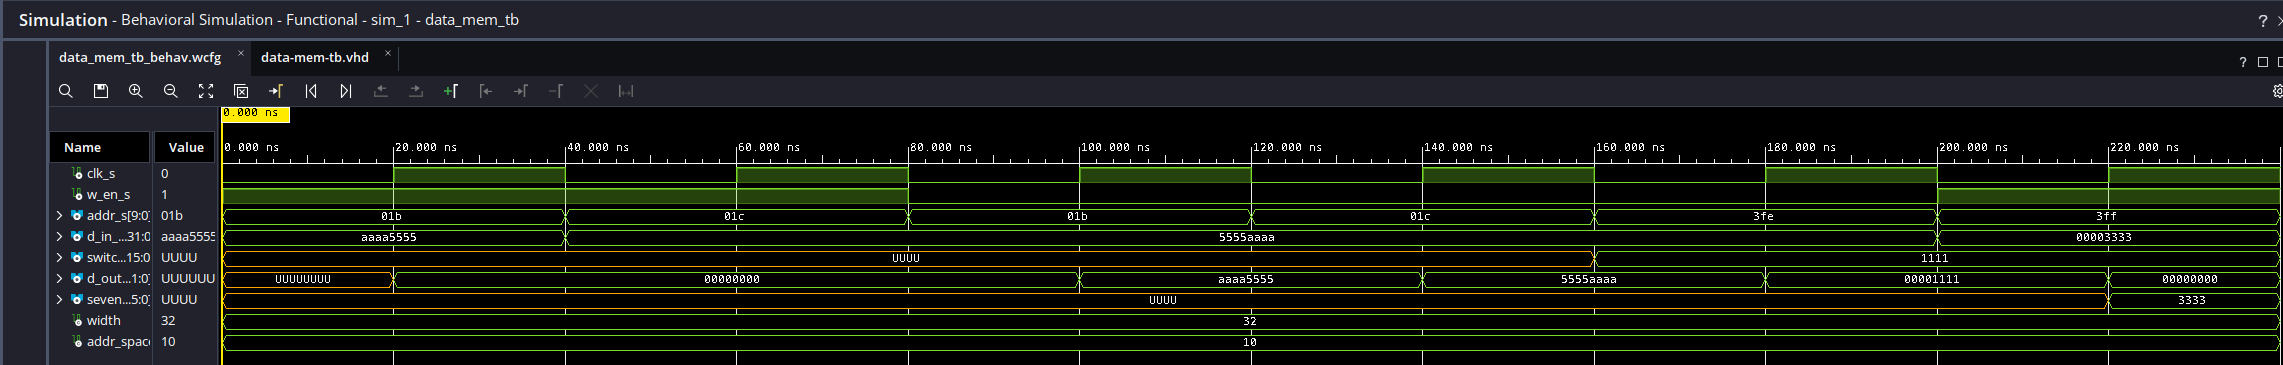
\includegraphics[width=\textwidth]{dmem-behv}
    \caption{Waveform for Behavioral Testbench for Memory Module}
    \label{fig:dmem-behv}
\end{figure}

The waveform given by Figure \ref{fig:dmem-behv} shows that all four test cases
passed. The design was implemented correctly.

It is especially important to verify that reading from address \texttt{0x3fe}
is successful; it is the only way to get external stimuli. The relevant test
case is given in Figure \ref{fig:dmem-behv-3fe}.

\begin{figure}[H]
    \center
    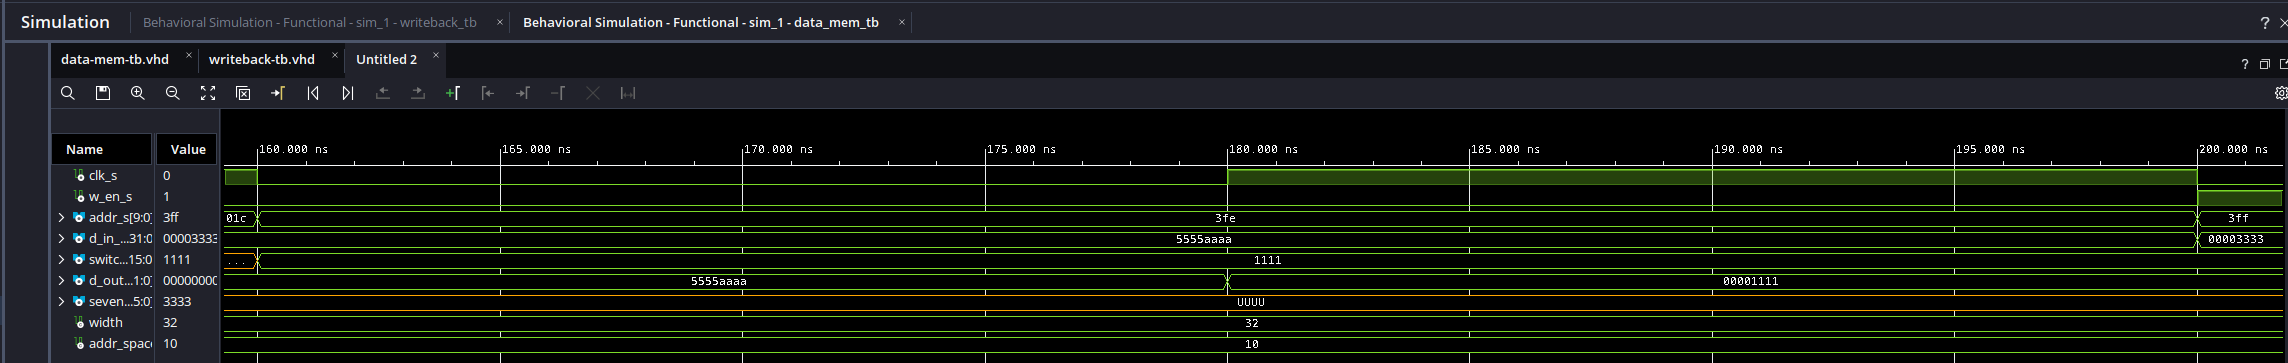
\includegraphics[width=\textwidth]{dmem-behv-3fe}
    \caption{Waveform for Reading from Switches}
    \label{fig:dmem-behv-3fe}
\end{figure}

The waveform in Figure \ref{fig:dmem-behv-3fe} gives the test case from 160 --
200 ns. The switch input is set every fourth switch active, and the address to
read from is set to \texttt{0x3fe}. On the rising clock edge, the output signal
becomes the switch input, backfilled with 0s. This is the desired behavior for
reading from the switch input address. The test case passed.

It is equally important to verify that writing to the address \texttt{0x3ff}
is successful; it is the only way to output data from the FPGA. The relevant
test case is given in Figure \ref{fig:dmem-behv-3ff}.

\begin{figure}[H]
    \center
    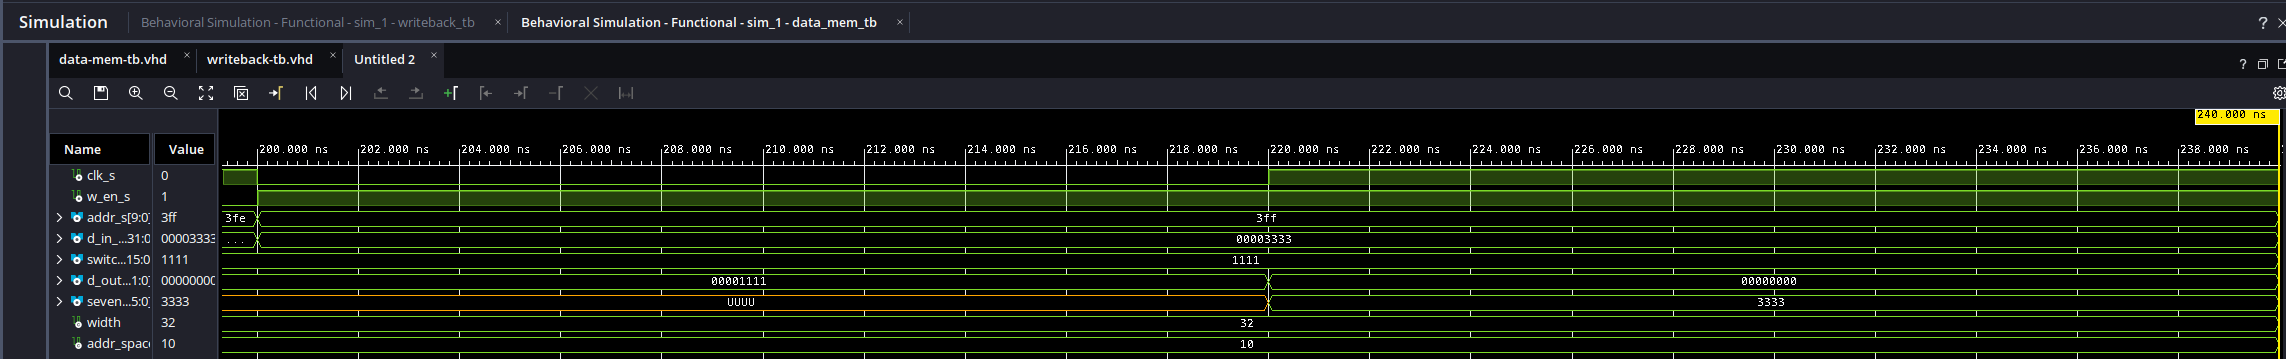
\includegraphics[width=\textwidth]{dmem-behv-3ff}
    \caption{Waveform for Writing to Display}
    \label{fig:dmem-behv-3ff}
\end{figure}

The waveform in Figure \ref{fig:dmem-behv-3ff} gives the test case from 200 --
240 ns. The address \texttt{0x3ff} is written to with the value
\texttt{0x3333}, backfilled with 0s. On the rising clock edge, the output
signal is cleared and the seven segment signal is set to \texttt{0x3333}. The
former indicates that the address does not store data. The latter indicates
that data sent to the address will be redirected to the seven segment display.
This is the desired behavior for writing to the display output address. The
test case passed.

To ensure the design remained correct when implemented in hardware, a
post-implementation timing simulation was run. The generated waveform is given
in Figure \ref{fig:dmem-pimp}.

\begin{figure}[H]
    \center
    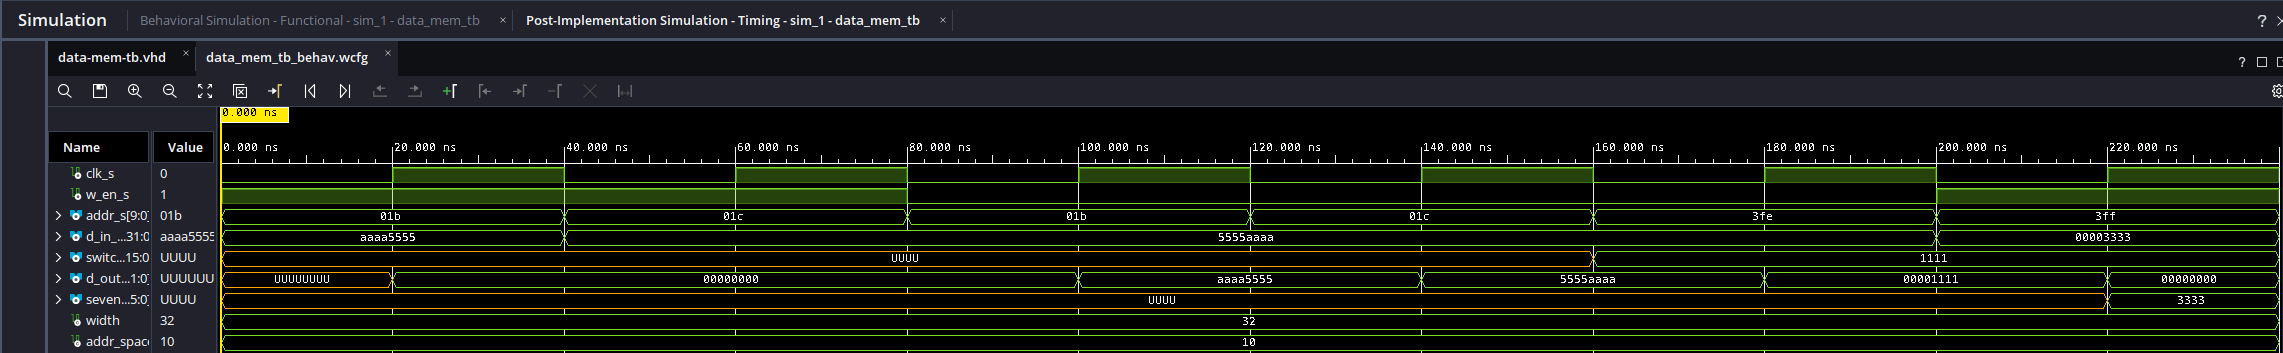
\includegraphics[width=\textwidth]{dmem-pimp}
    \caption{Waveform for Post-Implementation Testbench for Memory Module}
    \label{fig:dmem-pimp}
\end{figure}

No significant or noticeable differences in timings were observed in Figure
\ref{fig:dmem-pimp}. This is likely due to the simplicity of the logic used to
determine outputs after the clock edge; in all cases, either direct assignment
or a mux is used. Because no significant differences were observed between the
post-implementation timing simulation and the behavioral simulation, the
post-implementation testbench passed.

In order to verify the correctness of the writeback stage, a testbench was
constructed that contained eight test cases. The testbench ensured correctness
in forwarding each signal, as well as in selecting correctly between the ALU
result and the memory output. The waveform generated by the behavioral
simulation is given in Figure \ref{fig:wb-behv}.

\begin{figure}[H]
    \center
    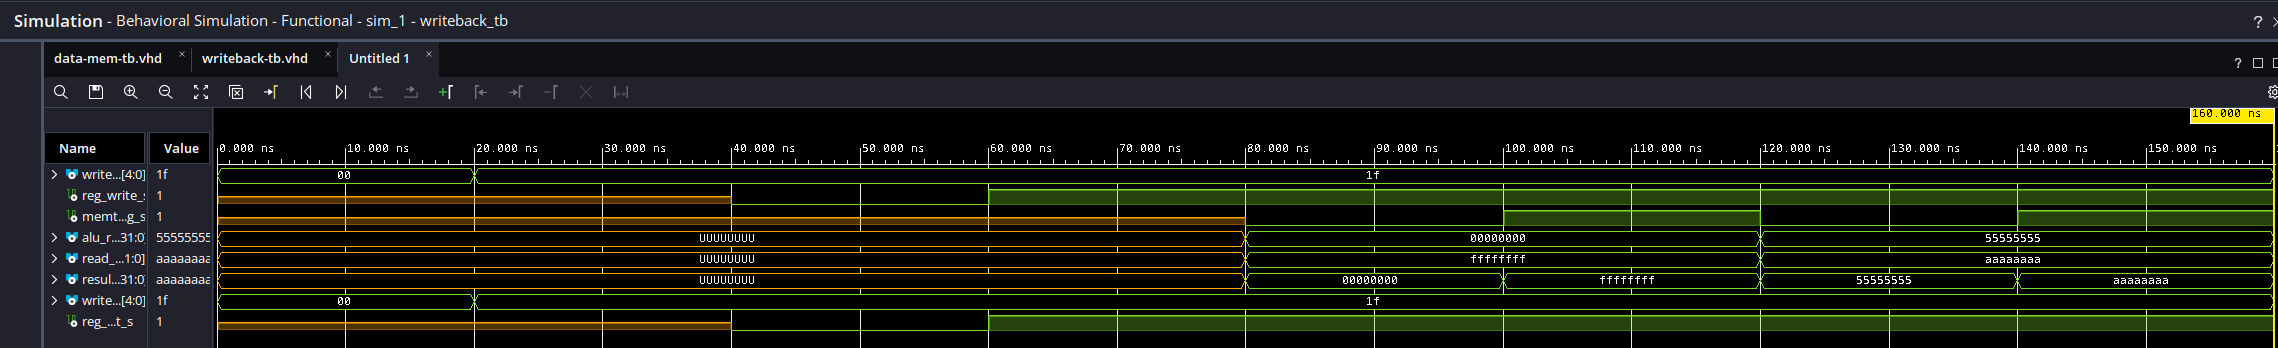
\includegraphics[width=\textwidth]{wb-behv}
    \caption{Waveform for Behavioral Testbench for Writeback Stage}
    \label{fig:wb-behv}
\end{figure}

The waveform given by Figure \ref{fig:wb-behv} shows that all eight test cases
passed. The design was implemented correctly.

The most important test cases are those that test the selection of the ALU
result versus the memory output. The selection logic is the most complex part
of the writeback stage. The waveform for a test case that ensures the ALU
result is picked is given in Figure \ref{fig:wb-behv-alu}.

\begin{figure}[H]
    \center
    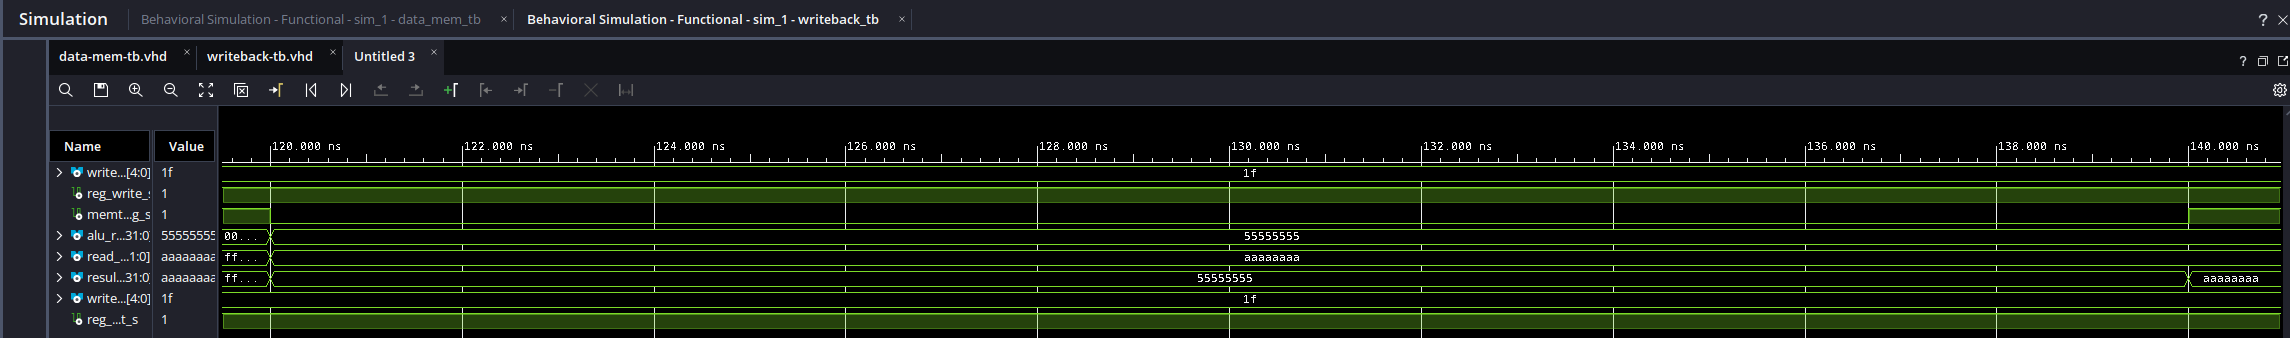
\includegraphics[width=\textwidth]{wb-behv-alu}
    \caption{Waveform for Selecting ALU Result}
    \label{fig:wb-behv-alu}
\end{figure}

The waveform in Figure \ref{fig:wb-behv-alu} gives the test case from 120 --
140 ns. The ALU result was set to all 5s and the memory output was set to all
As. The mem to reg signal was set to 0, indicating that the ALU result should
be used for output. The output signal was all 5s. This is the desired behavior
for selecting the ALU result. The test case passed.

It is equally important to ensure that the memory output can be selected. The
waveform for a test case that ensures the memory output is selected is given in
Figure \ref{fig:wb-behv-mem}.

\begin{figure}[H]
    \center
    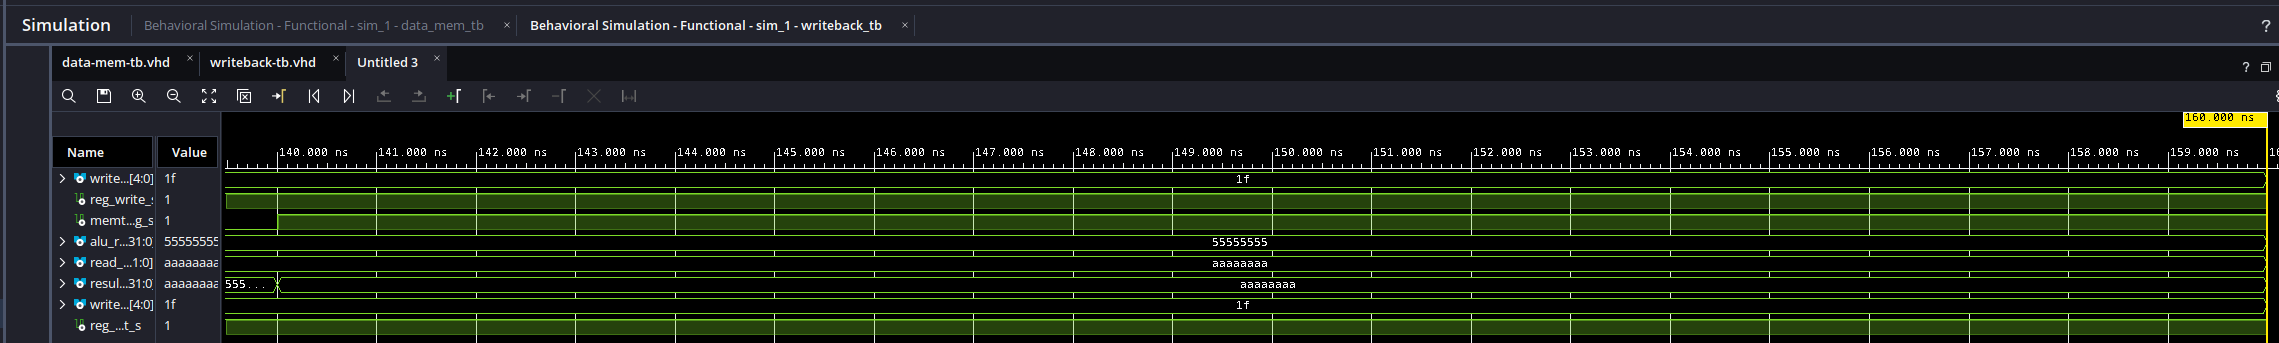
\includegraphics[width=\textwidth]{wb-behv-mem}
    \caption{Waveform for Selecting Memory Output}
    \label{fig:wb-behv-mem}
\end{figure}

The waveform in Figure \ref{fig:wb-behv-mem} gives the test case from 140 --
160 ns. The ALU result was set to all 5s and the memory output was set to all
As. The mem to reg signal was set to 1, indicating that the memory output
should be used for output. The output signal was all As. This is the desired
behavior for selecting the memory output. The test case passed.

\section*{Conclusion}
\addcontentsline{toc}{section}{Conclusion}

The objective of this exercise was to design memory and writeback stages to
store data in memory and interact with hardware. This was accomplished by
analyzing, translating to VHDL, and expanding upon partial Verilog
implementations of these stages. All testbenches for both stages passed, and
both implementations satisfied all design constraints and goals. The skills
needed to parse and understand other's code were shown to be useful in speeding
up development time; additionally, knowledge of Verilog was shown to be
necessary in understanding other's code. In future projects, Verilog may be
used instead of VHDL because it often has more concise syntax.


\includepdf[pages=-]{assets/prelab}
\end{document}
